\section{Full-day evidence with and without taker identifiers}

\paragraph{Independent samples.}
Before retrieving the extension panels, we fixed two calendars. On Binance we use the original three assets on the first day of every month in 2025. None of these 36 asset-days overlaps an original asset-day. On Coinbase we use BTC-USD, ETH-USD and SOL-USD throughout March 1, June 1, September 1 and December 1. These dates are disjoint from the short labelled windows. The replay archive keys its slices by capture time. We assign each match to its UTC capture hour, order by trade ID within product and hour, deduplicate identical IDs and retain exchange timestamps for the sweep rules. We use all 144 ten-minute slices of each day, concatenate adjacent slices before grouping executions, and cut at hour boundaries or missing trade IDs. The high and low groups are fixed from observed fill counts using the same six-hour rule on each venue. After opening these outcomes, we repeated the same design on the four corresponding days of 2024. The two years are reported separately. Group membership and the proposed ranking are observable after within-price aggregation. Coinbase identifiers provide the subsequent between-record reference labels. Sampling individual boundaries would require access to identifiers or an equivalent adjudication source.

The monthly Binance replication covers 64,754,885 fills and 18,357,619 records in 864 uninterrupted asset-hours. All 36 record-level rankings put the busiest hours higher, and 24 keep that sign over all native-time partitions. The result divides by asset (Table~\ref{tab:monthly}). Every SOL and LTC ranking survives, whereas each ETH interval contains both signs. As a fraction of daily records, the median native join capacity is 49.7\% for ETH, 5.5\% for SOL and 7.8\% for LTC. Many more boundaries are ambiguous on the ETH tape. With the more permissive 20 ms total span, all 36 intervals include both signs. Limiting the native-rule excess eligible-join fraction in the winning group to ten percentage points preserves 35 of 36 rankings. This is a sensitivity restriction on Binance, where the required fractions are latent.

On the 2025 labelled panel, the aggregate-record ranking disagrees with the consecutive taker episodes for March ETH and June BTC and ETH (Figure~\ref{fig:cb}). All three occur on dates with contiguous trade IDs. For June ETH the busy group contains 60,157 aggregate records from 34,004 labelled episodes. The quiet group contains 25,146 records from 16,983 episodes. Thus one episode has 1.77 records on average in the busy group and 1.48 in the quiet group. For a state with $n$ true episodes the excess same-side frequency when counting $M$ records is exactly $S(M-n)/[(n-J)(M-J)]$. The difference between these two state-specific excesses is 3.77 percentage points. It is sufficient to turn a labelled $-0.34$ point contrast into a record-level $+3.43$ point contrast.

The ETH and SOL markets share four dates across the two venues. For SOL, both the Binance identified sign and the observed Coinbase label sign are positive on each date. For ETH, the Binance native intervals allow either sign on all four dates and the Coinbase tape exhibits both directions. Magnitudes and state assignments are venue-specific. On June 1 even the Coinbase SOL contrast of $+0.51$ points falls below the Binance lower endpoint of $+2.95$ points. A label panel on a different exchange can check a measurement procedure without providing the latent value for the first venue.

The two activity groups can use nearly identical fractions of their potential joins and still switch places. In the twelve 2025 native comparisons the median absolute gap between their observed fractions is 0.091 percentage points and the maximum is 0.296 points. For each of the three observed record-to-label reversals, the minimum required positive excess under the native rule is zero. The fraction of records that \emph{can} be joined may differ sharply across states even when the propensity to take an eligible join is similar. Off-rule joins are separately counted in the released diagnostics. Imposing a common uptake fraction without inspecting the two states' capacities would miss this distinction.

\paragraph{Temporal replication and the activity definition.}
The 2024 panel again yields three record-to-label reversals in twelve comparisons. In March the busy ETH group leads by 0.71 points on records but trails by 2.34 points on episodes. The March BTC and September SOL rankings also reverse. Native greedy grouping recovers the label direction in all twelve 2024 comparisons and eleven in 2025. The median absolute error in the contrast falls from 1.48 to 0.003 points in 2024 and from 1.36 to 0.011 points in 2025. Across both years all eighteen labelled contrasts with magnitude above one percentage point have the correct native-greedy sign. These are descriptive same-tape comparisons of estimators.

Across the two yearly panels the archive contains 7,757,817 observed fills and 4,527,124 labelled episodes. There are 33 within-hour discontinuities spanning 301 missing trade IDs, and 120 observed fills lie outside their capture hour by exchange time. An independent replay using trade ID, taker ID and side reproduces the observed label numerator and denominator in all 576 asset-hours. Dropping hours with gaps before choosing states preserves all six record-to-label reversals. Equal weighting of hours within the original states also preserves the same six. The sole native-greedy sign disagreement in September 2025 survives the gap-free check but disappears under equal hour weights.

An exploratory check redefines activity as the number of labelled episodes and selects the six busiest and quietest hours afresh. Four record-to-label reversals occur in 2024 and one in 2025 under that definition. Thus fragmentation can affect both the assignment of states and their persistence ranking. The primary exercise fixes a fill-based activity definition that is observable on an anonymous tape.

\begin{table}[htbp]\centering\small
\caption{Previously unexamined Binance asset-days under native-time grouping. Counts refer to asset-days except in the final column.}\label{tab:monthly}
\begin{tabular}{lrrrrrr}\toprule
Asset & Days & Rows $+$ & Greedy $+$ & Identified & Cap 10 pp & Median $k$\\\midrule
\tableinput complete-monthly.tex
\bottomrule\end{tabular}
\smallskip

\begin{minipage}{.94\linewidth}\footnotesize
Rows and Greedy count positive high-minus-low contrasts at the aggregate and maximal-join partitions. Identified counts contrasts whose bounds exclude zero in either direction. Cap 10 pp allows the row-level winner's eligible join fraction to exceed the loser's by at most ten percentage points. Median $k$ gives the boundary checks needed for the greedy ranking under (\ref{eq:audit}) with 5\% risk and zero discrepancies.\end{minipage}
\end{table}

\begin{figure}[htbp]\centering
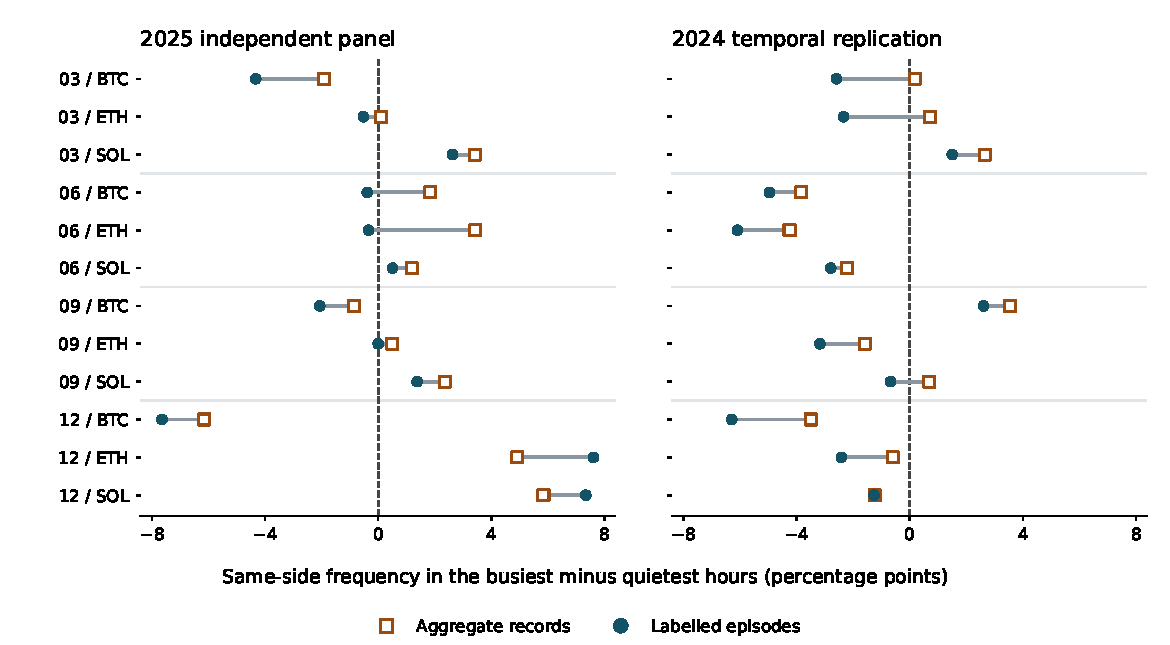
\includegraphics[width=\linewidth]{full-day-ranks.pdf}
\caption{Full-day Coinbase activity contrasts by month and asset. Points connected across zero imply opposite state rankings on the same tape. The busiest and quietest hours always use the same underlying fills within each comparison.}\label{fig:cb}
\end{figure}

\paragraph{Audit costs and observed boundary errors.}
Use the native-time maximal-join ranking as the proposed order. In 2025 the labelled number of harmful errors is below $b^*$ in eleven of twelve comparisons. The exception is September ETH, for which the greedy contrast is $-0.01025$ percentage points and the observed label contrast is $+0.00074$. Only 16 harmful edits are needed to eliminate that greedy ranking, and the census finds 59. An audit on this tape needs 14,018 clean boundary checks for a 5\% certificate. The exact probability of passing the zero-hit procedure with these actual errors is $0.000016$. This near tie is informative about verification cost even though its sign has little economic consequence.

For each labelled tape we compute the probability of certification as $\binom{N-e}{k}/\binom{N}{k}$ using its complete count $e$ of harmful discrepancies. These are operating characteristics over possible samples, calculated without fitting or simulating a boundary-error distribution. In the 2025 native panel the median required targeted sample is 66 and the median success probability is 97.2\%. The all-same-side benchmark takes a median 130.5 checks. Under a per-family 5\% Bonferroni adjustment for the twelve native comparisons, the median targeted sample rises to 121 and the median probability falls to 95.0\%. A failure to certify can occur on a correctly ranked tape: June ETH has the correct native sign but a zero-hit probability of only 15.0\%. Under millisecond rounding the median 2025 success probability falls to 45.4\% (Table~\ref{tab:cost}). The extra merging opportunities increase the number of distinct-episode edges admitted by the greedy rule.

In the 2024 replication the native rule needs a median of 68 checks, against 134 from all same-side boundaries, and its median zero-hit probability is 99.3\%. The observed harmful errors are below the exact margin in every cell. Millisecond grouping has the correct sign in all twelve cells but only a 59.6\% median chance of certification at its minimal budget. Correct rankings and easy-to-verify rankings can diverge. On the anonymous monthly Binance panel the corresponding native sample sizes range from six to 285 checks. These last counts describe a design an exchange could implement if it supplied reliable taker labels for the selected edges.

\begin{table}[htbp]\centering\small
\caption{Verification performance with a complete Coinbase label census. Each group of 12 reported rankings has a separate family-wise sensitivity check in the archive.}\label{tab:cost}
\begin{tabular}{llrrrrr}\toprule
Year & Rule & Sign matches & $e<b^*$ & Targeted $k$ & All-edge $k$ & Cert. prob.\\\midrule
\tableinput audit-performance.tex
\bottomrule\end{tabular}
\smallskip

\begin{minipage}{.95\linewidth}\footnotesize
Sign matches compare the greedy ranking with the labelled ranking. $e$ counts observed errors in the two harmful classes. $b^*$ is their minimum required for a tie or reversal. Remaining columns give the median per-comparison 5\% zero-hit budgets under the two sampling frames and the median probability of certification with the targeted budget.\end{minipage}
\end{table}
